%
%  Vincent Yannello
%
\documentclass[12pt,fullpage]{article}
\usepackage{fullpage}
\usepackage{psfrag}                                          % LaTeX graphics tool
\usepackage{pslatex}                                         % avoids the default cmr font
\usepackage{graphicx}                                        % graphics package 
\usepackage{epsfig}                                          % figures
\usepackage{hyperref}
\usepackage{color}

\begin{document}

\noindent
{\bf TSP distribution} (from \color{blue}\url{http://www.math.wm.edu/~leemis/chart/UDR/UDR.html}\color{black})

\noindent
The shorthand $X \sim {\rm TSP}(a,\, b,\, m,\, n)$ is used to indicate that the
random variable $X$ has the TSP distribution with parameters $a$, $b$, $m$, and $n$.
A TSP random variable $X$ has probability density function 
$$
f(x) = \left\{ \begin{array}{ll}
		\frac {n\, \left( x - a \right) ^ {n - 1}}{ \left( b - a \right) 
 \left( m - a \right) ^ {n - 1}} & \qquad a < x < m \\
		\frac {n \, \left( b - x \right) ^
{n - 1}} { \left( b - a \right)  \left( b - m \right) ^ {n - 1}} & \qquad m \leq x < b,
		\end{array} \right. \, 
$$
for $n > 0$, and $a < m < b$. The probability density function with $a = 0, b = 8, m = 3,$ and $n=4$ is illustrated below.

\begin{figure}[h!]
\begin{center}
\psfrag{labx}{$x$}
\psfrag{labf}{$f(x)$}
\includegraphics[width=3.2in]{TSPPlot.ps}
\end{center}
\end{figure}

\noindent		
The cumulative distribution function on
the support of $X$ is 
$$
F(x) = P(X \le x) = \left\{ \begin{array}{ll}
		\frac { \left( x - a \right) ^ {n} \left( m - a \right) ^ {1-n}}
{b - a} & \qquad a < x < m \\
		- \frac {a + b(b - x)^n(b-m)^{-n} - b - m(b-x)^n(b-m)^{-n}}{
b - a} & \qquad m \leq x < b.
		\end{array} \right. \, 
$$
The survivor function on the support of $X$ is
$$
S(x) = P(X \ge x) = \left\{ \begin{array}{ll}
		-\frac {-b + a +\left( x - a \right) ^ {n} \left( m - a \right) ^
{1 -n}}{b - a} & \qquad a < x < m \\
		\frac { \left( b - x \right) ^ {n} \left( b - m
 \right) ^ {1 -n}}{b - a} & \qquad m \leq x < b.
		\end{array} \right. \, 
$$
The hazard function on the support of $X$ is
$$
h(x) = \frac{f(x)} {S(x)} = \left\{ \begin{array}{ll}
		-\frac {n \, \left( x - a \right) ^ {n - 1} \left( m - a \right) ^
{1-n}}{a - b +  (m - a)
 \left( x - a \right) ^ {n} \left( m - a \right) ^ {-n}}  & \qquad a < x < m \\
		{\frac{n}{b - x}} & \qquad m \leq x < b.
		\end{array} \right. \, 
$$
The moment generating and characteristic functions of $X$ are mathematically intractable. The population mean and variance of $X$ are
$$
E[X] = {\frac {b - m + m \, n + a}{n + 1}} \quad \quad 
$$
$$
V[X] = {\frac {-2 \, m \, n \, b + 2 \, {m} ^ {\kern 0.08 em 2} n + {a} ^ {\kern 0.08 em 2} n + {b} ^ {\kern 0.08 em 2} n - 2 \, m \, n \, a + 2 \, b \, m - 2
\, b \, a + 2 \, a \, m - 2 \, {m} ^ {\kern 0.08 em 2}} { \left( n + 1 \right) ^ {\kern 0.08 em 2} \left( n + 2
 \right) }}. \quad \quad 
$$

\vspace{0.05in}

\noindent
{\bf APPL verification:}
The APPL statements
\begin{verbatim}
X := [[x -> (n * (x - a) ^ (n - 1)) / ((b - a) * (m - a) ^ (n - 1)),
       x -> (n * (b - x) ^ (n - 1)) / ((b - a) * (b - m) ^ (n - 1))],
      [a, m, b],["Continuous", "PDF"]];
CDF(X)
SF(X);
HF(X);
Mean(X);
Variance(X);
Skewness(X);
Kurtosis(X);
\end{verbatim}
verify the cumulative distribution function, survivor function, hazard function, population mean, variance, skewness, and kurtosis.

\end{document}
